%!TEX root = thesis.tex

\chapter{Sonic Gesture}
\label{ch:sonicgesture}

\section{Implementation}
\label{sec:implementation}

\begin{figure}[ht]
\centering{}
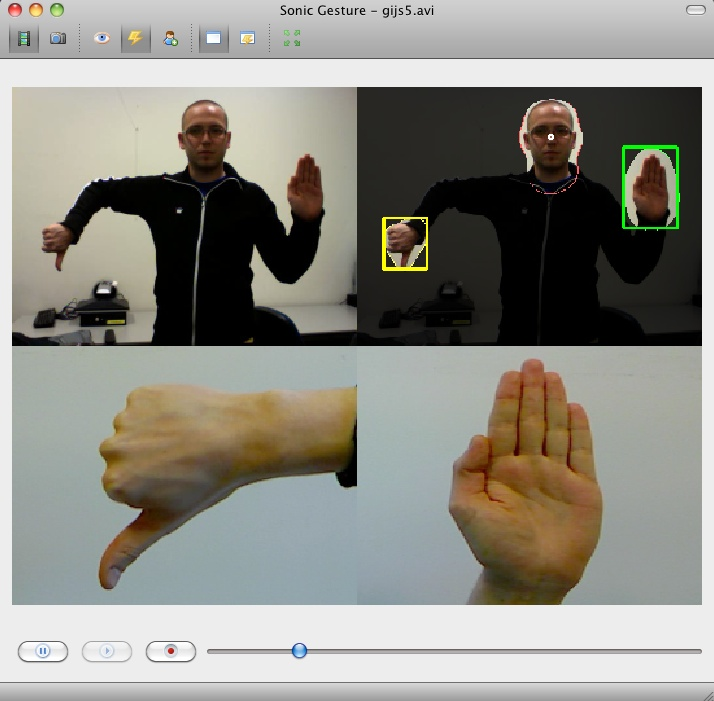
\includegraphics[width=0.6\linewidth]{figures/sonicgesture.jpg}
\caption{Screenshot of Sonic Gesture}
\label{fig:sonicgesture}
\end{figure}

Sonic Gesture has been implemented in C++. Almost all computer vision algorithms used are part of OpenCV, an open source library made for this kind of software. For the graphical interface QT is used. Sonic Gesture has been release as Open Source software and is released under the Apache license. The software can be downloaded, modified and distributed freely from the website\footnote{http://code.google.com/p/sonic-gesture}.

\autoref{fig:sonicgesture} is a screenshot of the main screen of sonic gesture. The program can capture directly from a webcam or it can read movies with recorded material. It has 2 modes, the first is the `finder' mode where hand poses in the video stream are detected and classified. The second mode is the `capture' mode, which is used to label movies. When labeling a movie in this mode a text file is created with frame positions of the labels. This can later be used to extract the correct frame and extract training data for the classifier. This mode has been used a lot during the gathering of the dataset.

When the finder mode is active, Sonic Gesture will translate the labeled hand poses, the hand positions and the size of the hand into Open Sound Control (OSC). OSC is a protocol which is specially designed for transferring audio information over a network. For those who are familiar with digital music, it is very similar to MIDI. A program that can interpreted OSC can then be configured to listen on a specific port and process these OSC command.

Sonic Gesture will submit
\begin{itemize}
	\item For each hand the beginning and the end of detected sequence of hand specific hand pose. This is an integer. This can be used to trigger a action, like playing a specific note.
	\item The position of each hand in $x$ and $y$ position. This is a float and can be used to manipulate a parameter.
	\item The size of the hand. This is also a float and can also be used to manipulate a parameter.
\end{itemize}

There is no strict defined relationship between a hand pose and a sound or parameter, the user of Sonic Gesture can define his own specific mapping with his or her preferred audio application. 

\section{Time Performance}
A lot of effort has been put into getting Sonic Gesture as fast as possible. Initially Sonic Gesture was written in Python and used the Python API of OpenCV. Soon it became clear that Python was to limited to do high performance graphic processing so a switch to C++ was made. 

The performance of Sonic Gesture depends on how fast the testing systems CPU power is, if the OpenCV IPP extention is used but also how fast the camera can capture frames. On a Macbook Pro, 2.4 GHz intel core 2 duo with 4 GB of memory using the build-in iSight as camera, processing one frame takes 65 ms on average. This is with the full dataset of 2072 datapoints with 3780 dimensions using the KNN classifier. KNN works fine with low numbers of datapoint, but with high numbers it starts to slow down. Still it is quite fast; around 25 ms on average. SVM will probably perform much faster with a high number of datapoints but we couldn't get the SVM implementation of OpenCV to work. An other expensive operation is the face detection algoritm, when tweaked it takes around 13 ms to locale a face in a image. Since a face position is not required constantly this is done only every 10th frame, so valuable computation time is saved. An other surprisingly expensive operation is the resizing of a image. Resizing an image to a small size is a crucial part of the pipe line, because some operations on a big image will take too much time. But resizing a image using interpolation is a expensive operation. Where interpolation is not required, for example for rendering on the screen, it is disabled saving more computing time. 



\begin{table}
\centering
\begin{tabular}{cccc}
What & relative time & absolute time & comment \\
\hline
kNN & 47\% & ... & 3780 features, 2016 samples \\
Color space convertion & 8.4\% & ... & \\
Image resizing & 7.6\% & ... & \\
Face detection & 3.7\% & ... &  19\% if every frame \\
HOG features & 2.6\% & ... \\
\end{tabular}
\caption{Performance timing of Sonic Gesture}
\end{table}

calculating SURF features of a hand train image takes 4ms and results in 11 features on average.